% Contributers: Noah Huber-Feely, Samuel Sharpe
\subsection{(1+$\epsilon$)-approximate $k$-means clustering}

Unlike Lloyd's method, this approximation algorithm guarantees that it will have
a cost no more than (1+$\epsilon$)-times the true minimum cost and will do so in
in time O($n$ log$^k$ $n$) for any $\epsilon>0$. This method uses intelligent
preprocessing of the space to achieve this result. Formally, we define
$\Pi = (S_1, S_2, ..., S_k)$ to be some partitioning of an $n$-point set
$X \subset \bbR^d$ for some number $k \geq 2$. Further, cost($\Pi$)=$\sum_{i=1}^k \text{cost(}S_i)$ where cost($S$)=
$\sum_{x \in S} ||x-c(S)||^2$. Here $c(s)=(1/|S|) \sum_{x \in S} x$ and is
thus the centroid of the set $S$. Let diam($X$) denote the diameter of a set
$X \subset \bbR^d$. Further, this and other centroid base clustering methods relies upon the Vornoi partition of a set of points by the centroid points.
For centroids $c_1,...,c_k$, we refer to the Vornoi partition $(S_1,S_2,...,S_k)$ of a set
as $\Pi_{Vor}(c_1, c_2, \dots, c_k))$.

We say that a $k$-clustering $\Pi$ of $X$ is (1 + $\epsilon$)-approximately optimal if cost($\Pi$) $\leq$ (1 + $\epsilon$)cost($\Pi'$) for any $k$-clustering $\Pi'$ of $X$. The method described below thus achieves the results outlined in the following two theorems.

\begin{theorem}
Let $X \subset \bbR^d$ be an n-point set, and let $\epsilon >0$ be given. A (1 + $\epsilon$)-approximately optimal 2-clustering of X can be found in time $O(n\text{ log }n \cdot \epsilon^{-2d} \text{log }\frac{1}{\epsilon} + n \epsilon^{-(4d-2))}\text{log }\frac{1}{\epsilon})$ so the running time is $O(n\text{ log }n)$ for a fixed $\epsilon>0$.
\end{theorem}

\begin{theorem}
Let $X \subset \bbR^d$ be an n-point set, let $k \geq 3$ be fixed and let $\epsilon >0$ be given. A (1 + $\epsilon$)-approximately optimal k-clustering of X can be found in time $O(n(\text{log }n)^k \epsilon^{-2k^2d})$.
\end{theorem}

We thus see that we achieve a near-linear time algorithm for both (1 + $\epsilon$)-approximate 2-means and k-means.

This approach requires some additional preliminary terminology and cost definitions which are themselves interesting ideas for this problem space.
\begin{definition}[$\epsilon$-near]
Let $\epsilon \geq 0$. We define $\sim_{\epsilon}$ to be a relation on ordered pairs of points in $\bbR^d$. We say that $(x,y)$ and $(x',y')$ are $\epsilon$-near if $(x,y) \sim_{\epsilon} (x', y')$ such that  $(x,y) \sim_{\epsilon} (x', y')$ if $||x-x'|| \leq \epsilon \cdot ||x-y||$ and $||y - y'|| \leq \epsilon \cdot ||x - y||$.
\end{definition}

\begin{definition}[$\epsilon$-separated]
Let $P$ be a set of ordered pairs of points of $\bbR^d$. We say $P$ is $\epsilon$-separated if no two pairs in $P$ are $\epsilon$-near.
\end{definition}

\noindent \emph{Approximate range searching}. An important and useful concept for optimizing this problem is approximate range searching. At a high level, this method uses intelligent preprocessing to attempt to find an approximate answer to the weight sum within a specific range for a set $P \subset \bbR^d$ where each point is assigned a weight such that for $p \in P$, $w(p) \in S$ where $S$ is a commmutative semigroup (meaning weights can be summed). Formally, given a range $R \in \cR$ where $\cR$ is a class of admissible ranges and some $\epsilon>0$, we define $R^+$ to be the set of all points at most a distance of $\epsilon \cdot$diam($R$) from $R$, and let $R^-$ be all points of distance at most $\epsilon \cdot$diam($R$) from the complement of $R$.

\begin{definition}[$\epsilon$-approximate intersection]
Let $P$ be a an $n$ point subset of $\bbR^d$ and let $R$ be a range. Then an $\epsilon$-aproximate intersection of P with a range R is any subset $P_1 \subseteq P$ with $P \cap R^- \subseteq P_1 \subset P \subseteq R^+$.
\end{definition}

\begin{definition}[$\epsilon$-approximate answer]
An $\epsilon$-approximate answer to the query with range $R$ is any weight of the form $\sum_{p \in P_1} w(p)$, where $P_1$ is any $\epsilon$-aproximate intersection of $P$ with $R$.
\end{definition}

This method takes $O(n\text{ log }n)$ preprocessing time and can then produce an $\epsilon$-approximate answer in $O(\text{log}n + \epsilon^{-d})$ as shown by Arya and Mount.

\noindent \emph{Putting the points on a polynomial-size grid}. The proposed k-clustering problem works with points with polynomially large distances between them, however ratios of interpoint distances can be arbitrarily large. The set of points $X$ can be 'snapped' onto a integer grid with polynomial size (specifically $O(n^3/\epsilon)$). If there is some algorithm that can compute an $(1+\epsilon)$-approximate clustering for $X'$. Then a $(1+\epsilon)$-approximate clustering for the arbitrarily large $X$ can be computed with $O(nlogn)$ processing time. This is tangential to the main result so we do not present the proof here. Now we proceed assuming the n-point set $X \subset \bbR^d$ lie on an integer grid of size $O(n^3/\epsilon)$.\\

\noindent \textbf{Approximate Centroid Sets}\\
Let $S$ be a finite set in $\bbR^d$. The quadratic-mean radius of S is
\begin{align}
    \rho(S)  = \left( \frac{1}{|S|}\sum_{x\in S}\norm{x-c(S)}^2\right)^{1/2}
    = \sqrt{\frac{cost(S)}{\abs{S}}}
\end{align} 
be the \emph{quadratic-mean radius} of S. For a real number $\epsilon \geq 0$, the \emph{$\epsilon$-tolerance ball} of S is the ball centered as $c(S)$ of radius $(\epsilon/3)\rho(S)$.
\begin{definition}[$\epsilon$-approximate centroid set]
Let $X \subset \bbR^d$ and $C \subset \bbR^d$ be finite point sets. We call C an $\epsilon$-approximate centroid set for $X$ if $C$ intersects of the $\epsilon$-tolerance ball of each nonempty$ S \subseteq X$. If it intersects the $\epsilon$-tolerance ball  of each cluster size s or larger it is a $\epsilon$-approximate centroid set for X for cluster size $\geq s$.
\end{definition}

\begin{lemma}
Let $X \subset \bbR^d$ be a finite point set, let $k\geq 2$, and let $C$ be an $\epsilon$-approximate centroid set for $X$ for cluster size $\geq s$. Then there are $c_1, c_2, \dots, c_k \in C$ such that 
$$cost(\Pi_{Vor}(c_1, c_2, \dots, c_k)) \leq (1+\epsilon)cost(\Pi)$$
for any k-clustering $\Pi$ of $X$ with all clusters of size at least s. 
\end{lemma}
\begin{proof}
Let $(S_1, S_2, \dots, S_k)$ be an optimal $k$-clustering of $X$ with all clusters of size at least $s$. For $i = 1,2,\dots,k$ choose $c_i \in C$ lying in the $\epsilon$-tolerance ball of cluster $S_i$. We can bound the cost of each cluster $S_i$ given $c_i$ as the center:

\begin{align*}
    cost(S_i, c_i) & = \sum_{x \in S_i}\norm{x-c_i}^2 \leq \sum_{x \in S_i} (\norm{x-c(S_i)} + \norm{c(S_i)-x})^2  && \text{by triangle ineq} \\
    & = cost(S_i) + 2\norm{c_i-c(S_i)}\sum_{x \in S_i}\norm{x-c(S_i)} + \abs{S_i}\norm{c_i-c(S_i)}^2 \\
    & \leq cost(S_i) + 2\frac{\epsilon}{3}\rho(S_i)\sqrt{\abs{S_i}}\sqrt{cost(S_i)} + \abs{S_i}\left(\frac{\epsilon}{3}\rho(S_i) \right)^2 && \text{by cauchy-schwartz } \\
    & \leq cost(S_i) + \frac{2}{3}\epsilon cost(S_i) + \frac{\epsilon^2}{9}cost(S_i) \\
    & \leq (1+\epsilon) cost(S_i)
\end{align*}
Cauchy-Schwartz is applied above as
$$\left( \sum_{x \in S_i}1\norm{x-c(S_i)} \right)^2 \leq \abs{S_i}\sum_{x \in S_i}\norm{x-c(S_i)}^2 $$
$$ \sum_{x \in S_i}\norm{x-c(S_i)} \leq \sqrt{\abs{S_i}cost(S_i)} $$
Finally, if we choose $S_i'$ based on the Voronoi partition of $c_i$
where $(S_1', S_2', \dots S_k') =\Pi_{Vor}(c_1, c_2, \dots, c_k) $, by optimality of the Voronoi partition we have
$$\sum_{i=1}^k cost(S_i') \leq \sum_{i=1}^k cost(S_i', c_i) \leq \sum_{i=1}^k cost(S_i, c_i) \leq (1+\epsilon) \sum_{i=1}^k cost(S_i)$$
\end{proof}

\noindent \emph{Constructing $\epsilon$-approximate centroid set for $X$}. Now we construct an $\epsilon$-approximate centroid set, $C$ for $X$ with a polynomial number of points from which we can identify centroids for the (1+$\epsilon$)-approximate $k$-clustering. Given $X$ (on a integer grid of size $O(n^4)$), minimum cluster size $s$, $\epsilon >0$ and $\delta >0$ where $\delta$ is a lower bound on $\min\norm{x-y}$ for $x,y\in X$. We set $r = \delta/n$ though $\delta/\sqrt{2}$ is sufficient. For any cluster $S \subseteq X$ with at least two distinct points, $\rho(S)\geq r$. 
 $$\rho(S) = \sqrt{\frac{cost(S)}{\abs{S}}} = \sqrt{\frac{1}{2\abs{S}^2}\sum_{x,y \in X}\norm{x-y}^2} \geq \sqrt{\frac{1}{2\abs{S}^2}\sum_{x,y \in X}\delta^2} =  \delta/\sqrt{2}$$
 
To construct this set we will reference \emph{cubes} which are axis-parallel cubes in $\bbR^d$ and the $K$-enlargement of a cube is a concentric cube with a side $K$-times larger. We let $Q_0$ be the 3-enlargement of the smallest cube enclosing $X$, and $R$ be the side of $Q_0$. We define an \emph{active cube} as any cube containing at least $x/2^{d+1}$ points of X. We initially set $C = \emptyset$. 

\noindent The construction of C begins at each step by repeated subdivision of $Q$ into $2^d$ equal-sized axis aligned cubes. For any cube $Q$ that is active, we let $\sigma$ be the side length of $Q$ and choose $C_Q$ that is $(\frac{\epsilon }{18} \sigma)$-dense for the 2-enlargement of $Q$ (see Figure \ref{fig:cq}). We can say $|C_Q| = O(\epsilon^{-d})$. Finally, we add $C_Q$, to the constructed set C.  After this is done for $Q$, it is no longer active and is further subdivided as long as $\sigma \geq 2r$. We stop when there are no active cubes left. 

\begin{figure}
    \centering
    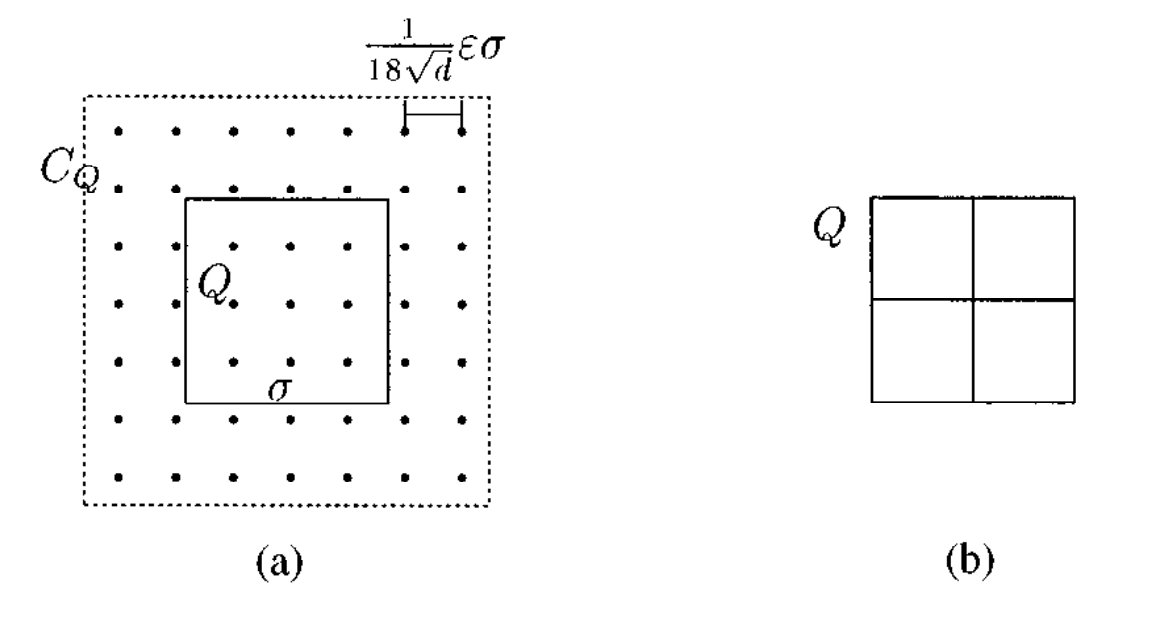
\includegraphics[width=10cm]{chapter_1/files/Cq.png}
\centering
    \caption{(a) The set $C_Q$ and (b) the subdivision of $Q$}
    \label{fig:cq}
\end{figure}

\begin{lemma}We have $\abs{C} = O((n/s)\epsilon^{-d}log(nR/\delta))$ and the construction can be formed in time $O((n+(n/s)\epsilon^{-d})log(nR/\delta))$. The constructed set C is an $\epsilon$-approximate centroid set for X for cluster size $\geq s$.
\end{lemma}
\begin{proof}
Since the minimum allowable size cube side length is $2r$ and we divide cubes by two in each dimension, we encounter active cubes with at most $O(log(R/r))$ distinct side lengths. Since there is a lower bound of $s/2^{d+1}$ points in each cube cubes are disjoint, the upperbound on active cubes is $O((n/s)log(nR/\delta))$. Finally, by the constructed density of $C_Q$ for each active cube the bound on size of C follows. 

\noindent To show that C is an $\epsilon$-approximate centroid set for X we show that $C$ intersects some of these active cubes and is sufficiently close to points in all clusters. We let $S \subseteq X$ be a cluster of size $\geq s$ with at least two points. By Markov's inequality, the ball B or radius $\sqrt{2}\rho(S)$ centered at $c(S)$ contains at least $s/2$ points of $S$. The statement follows from the probability that a given point $x$ is less than $\sqrt{2}\rho(S)$ away from a center:
\begin{align*}
    P(\norm{x-c(S)}^2 \geq 2\rho(S)^2) & \leq \frac{\frac{1}{|S|}\sum_{x\in S} \norm{x-c(S)}^2 }{2\rho(S)^2} 
\end{align*}
Let $j \geq 0$ be the integer sutch that $\sigma = R/2^j \in [3\rho(S),6\rho(S)]$. Since $diam(B) < \sigma$, B intersects at most $2^d$ cubes of side $\sigma$, so there must be a cube $Q$ that contains at least $s/2^{d+1}$ points of X and was active. The point $c(S)$ is at distance at most $\sqrt{2}\rho(S) \leq \sigma/2$ from $Q$, so it lies in the 2-enlargement of Q. Thus, $C_Q \subseteq C$ contains a point at distance at most $\frac{\epsilon}{18} \sigma \leq \frac{\epsilon}{3}\rho(S)$ from $c(S)$. Thus, C intersects the $\epsilon$-tolerance ball of S. 
\end{proof}

\begin{remark}
The authors provide a tighter bound on the size of C to $O(n\epsilon^{-d}log(1/\epsilon)$ and generalize the finding for any size cluster.
\end{remark}
\newpage
\noindent\textbf{Approximate 2-Clustering}
We will first address the easier subproblem of developing an $O(n \text{ log } n)$ (1+$\epsilon$) approximate 2-clustering. We provide a straight forward algorithm below.

\begin{algorithm}[H]
  \caption{(1+$\epsilon$) $2$-means algorithm:}
\begin{algorithmic} 
\STATE Compute an $\epsilon$-approximate centroid set C for X
\STATE Generate the set P of all pairs $(c_1, c_2)$ of distinct points of C
\FORALL {($c_1,c_2$) $\in$ $P$}
    \STATE Compute the Voronoi diagram and produce the hyperplane $h$ bisecting the segment $c_1 c_2$
    \STATE Compute the cost of the 2-clustering given by $h$
\ENDFOR
\STATE Return the 2-clustering with the smallest cost as determined above
\end{algorithmic}
\end{algorithm}

To get an $\epsilon$-approximate answer for an optimal 2-clustering, we don't need to inspect all pairs of distinct points of C.  An $\epsilon$-complete set (for ever pair in $X$ there is an $\epsilon$ near pair in the set) of pairs is sufficient for a $(1+\epsilon)$-approximation. 

\begin{lemma}
Let $c1, c2 \in \bbR^d$ be points, and let $c_1', c_2'$ be such that the pairs $(c_1,c_2)$ and $(c_1',c_2')$ are $\epsilon$-near, $\epsilon \leq \frac{1}{9}$. Let $\Pi = \Pi_{Vor}(c_1, c_2)$ be the clustering of $X$ by the bisecting hyperplane of $c_1$ and $c_2$, and let $\Pi' = \Pi_{Vor}(c_1', c_2')$. Then $cost(\Pi')\leq (1+ 6 \epsilon)cost(\Pi)$
\end{lemma}

\begin{proof}
Let $\Pi = (S_1, S_2)$ and $\Pi' = (S_1', S_2')$. Given the optimality of Voronoi
  clusters for given centroids, we need to show that the cost of a clustering
  given $\epsilon$-near centroids is $\epsilon$-approximate, i.e. $$cost(S_1', c_1)
  + cost(S_2' , c_2) \leq (1 + 6\epsilon)[cost(S_1, c_1) + cost(S_2 , c_2)]$$ This
  is the same as showing for each $x \in S_1' \backslash S_1$ we have $\norm{x-c_1}
  \leq (1+16\epsilon)\norm{x-c_2}$ and symmetric argument for $x \in S_2' \backslash S_2$.
  Since $x \in S_1'$, x must be closer to $c_1'$ than $c_2'$, $\norm{x-c_1'}\leq  \norm{x-c_2'}$.
  Let $\delta = \norm{c_1'-c_2'}$. By the triangle inequality and definition of $\epsilon$-near we have
\begin{align*}
    \norm{x-c_1} &  \leq \norm{x-c_1'} + \norm{c_1-c_1'} \\
    & \leq \norm{x-c_1'} + \epsilon \norm{c_1'-c_2'}\\
    & = \norm{x-c_1'} + \epsilon \delta \\
    & \leq \norm{x-c_2'}+ \epsilon \delta \\
    & \leq \norm{x-c_2} + \norm{c_2-c_2'} + \epsilon \delta \\
    & \leq \norm{x-c_2} + 2\epsilon \delta
\end{align*}
we also have by similar reasoning
$$\norm{x-c_2}\leq \norm{x-c_2'} - \epsilon \delta \leq \delta/2 - \epsilon \delta$$
which implies $\delta \leq \frac{2}{1-2\epsilon}\norm{x-c_2}\leq 3 \norm{x-c_2}$. Using the bound on $\norm{x-c_2}$ and $\delta$, we have $\norm{x-c_1} \leq (1+ 6\epsilon)\norm{x-c_2}$ as required. 
\end{proof}

% We have already shown that for an $\epsilon$-approximate centroid set, the cost of a Voronoi partition for some pair of centroids is at most $(1+\epsilon)cost(\Pi)$ where $\Pi$ is any $2$-clustering. As the algorithm performs an exhaustive search of all pairs of centroids in the computed $\epsilon$-approximate centroid set, it is clear that it will thus try the least cost pairing and thus satisifes the $(1+\epsilon)$ approximation requirement.

It remains to show that this algorithm can be performed in near-linear time. In a direct implementation of this algorithm, we must consider $|C|^2$ pairs $(c_1,c_2)$ and for each pair, we need $O(n)$ time for computing the cost of the corresponding $2$-clustering. The set $|C|$ has size $O(n \epsilon^{-d} \text{log}(1/\epsilon))$ thus implying $O(n^2)$ for a fixed $\epsilon$. However, we only need to consider an $\epsilon$-complete set of pairs of $P$ which has size $|P|=O(n \epsilon^{-d})=O(n)$.

Further, using approximate range searching, computing the approximate cost can be done in $O(\text{log }n)$ time (down from $O(n)$). As each preprocessing step takes at most $O(n \log n)$ and the main for loop takes $O(n \log n)$ for a fixed $\epsilon$, the algorithm can thus run in $O(n \log n)$.

The full k-clustering algorithm builds on the intuition of the 2-clustering version and employs a recursive approach for finding the $(1+\epsilon)$ approximate.

\begin{algorithm}[H]
  \caption{(1+$\epsilon$) $k$-means algorithm:}
\begin{algorithmic} 
\IF {$k=1$}
  \STATE return $X$ (as the single cluster) and $cost(X)$
\ENDIF
\FOR {$k^*=2,3,...,k$}
  \STATE generate a set $\cC^*$ of ordered $k^*$-tuples for $C$
  \FORALL {($c_1,c_2,....,c_{k^*}$) $\in$ $\cC^*$}
    \STATE Let ($X_1,X_2,...,X_{k^*}$)=$\Pi_{\text{Vor}}(c_1,c_2,...,c_{k^*})$ be
    the Voronoi partition of $X$, and let $C_i$ be the points of $C$ lying in the
    $\epsilon \omega$-neighborhood of $c_i$, where $\omega$ is the distance of
    the two closest points among $c_1,c_2,...,c_{k^*}$.
    \IF {$C_i = \emptyset$}
      \STATE Disregard the current $k^*$-tuple
      ($c_1,c_2,...,c_{k^*}$)
    \ELSE
      \FOR {$i=1,2,...,k^*$}
        \STATE Call the procedure recursively on $X_i$ and $C_i$, with
        the number of clusters $k_i$ running from 1 to $k-k^*+1$
      \ENDFOR
      \STATE One now has a $k_i$-clustering of $X_i$ for all the
      considered $k_i$.
      \STATE Find the combination
      ($k_1,k_2,...,k_{k^*}$),$k_1+k_2+...+k_{k^*}=k$ for which the
      $k$-clusting of $X$ obtained by combining the comptuer
      $k_i$-culsterings of the $X_i$'s has the smallest cost.
    \ENDIF
  \ENDFOR
\ENDFOR
\STATE For each $k^*$-tuple in $\cC^*$ with all the $C_i$ nonempty,
we know have a single k-clustering. Now return the k-clustering with
the smallest cost (minimum over all $k^*$-tuples and over all $k^*=2,3,...,k$.
\end{algorithmic}
\end{algorithm}

\begin{remark}
\textbf{The proof of running time for this method builds on the proof for approximate $2$-clustering and employs the recursive nature of the algorithm to go from $O(n \log n)$ for 2-clustering to $O(n (\log n)^k)$ for the $k$-deep recursion tree of the approximate $k$-clustering.}
\end{remark}

